\chapter{Results and Analyses} \label{chap:experiments}

\section*{}

In this chapter, we present some results of experiments done using the approach developed
(Chapter ~\ref{chap:chap4}) and with multiple datasets (with different characteristics).

We also present some experiments, made in order to understand which values are better
for some parameters, and in which situations they work better or worst.

\section{Interval size without segmentation}

To test which intervals of time get better results for predicting time series
used on the approach, a dataset containing real data from 26-09-2013 to
27-01-2014 was used. The interval sizes tested were: 4 hours, 6 hours, 8 hours,
12 hours and 24 hours.

For this test only the \emph{Volume Forecasting}(Section~\ref{subsec:volume_forecast}) phase, was used.

The time intervals used for the test were:
\begin{itemize}
\item case 1 - The results presented on table~\ref{tab:case1_interval} use
26-09-2013 to 26-11-2013 for training; 27-11-2013 to 25-01-2014 for validation;
\item case 2 - The results presented on table~\ref{tab:case2_interval} use
26-09-2013 to 26-12-2013 for training; 27-12-2013 to 25-01-2014 for validation;
\item case 3 - The results presented on table~\ref{tab:case3_interval} use
26-09-2013 to 31-12-2013 for training; 01-01-2014 to 25-01-2014 for validation;
\end{itemize}

For each one of the three cases the error of the
impressions volume forecasting for every test interval is shown.
In every case, the interval that got better results was the 12 hour interval
(minimum \emph{MASE}).

Additional errors values and graphs for this test are available on Appendix
~\ref{ap:case1} (for case 1), Appendix~\ref{ap:case2} (for case 2) and Appendix~\ref{ap:case3}
(for case 3).

\begin{table}[!ht]
\footnotesize
\begin{tabular}{c|ccccccccc}
              & 4h baseline & 4h allow drift & 4h     &  & 6h baseline & 6h allow drift & 6h     &  &  \\ \hline
$\sigma$ (Real Data) & \multicolumn{3}{c}{946.25}           &  & \multicolumn{3}{c}{1358.24}           &  &  \\
RMSE          & 690.87      & 562.80         & 562.80 &  & 945.70      & 742.57         & 742.57 &  &  \\
MASE          & 0.5227      & 0.4397         & 0.4397 &  & 0.3659      & 0.3003         & 0.3003 &  & 
\end{tabular}

\vspace{0.5cm}

\begin{tabular}{c|ccccccccc}
              & 8h baseline & 8h allow drift & 8h     &  & 12h baseline & \color{red}{12h allow drift} & 12h     &  &  \\ \hline
$\sigma$ (Real Data) & \multicolumn{3}{c}{1785.84}           &  & \multicolumn{3}{c}{2224.74}           &  &  \\
RMSE          & 1150.43     & 955.35         & 955.35 &  & 1555.01     & \color{red}{1233.82}     & 1233.82 &  &  \\
MASE          & 0.2712      & 0.2473         & 0.2473 &  & 0.2253      & \color{red}{0.1967}      & 0.1967 &  & 
\end{tabular}

\vspace{0.5cm}

\begin{tabular}{c|ccc}
              & 24h baseline & 24h allow drift & 24h  \\ \hline
$\sigma$ (Real Data) & \multicolumn{3}{c}{1946.70}     \\
RMSE          & 2448.97     & 2139.99        & 2139.99   \\
MASE          & 1.4338      & 1.2725         & 1.2725 \\
\end{tabular}

\vspace{0.5cm}

\caption{Case 1: Forecast errors for different interval sizes (best result in
red)}\label{tab:case1_interval}
\end{table}




\begin{table}[!ht]
\footnotesize
\begin{tabular}{c|ccccccccc}
              & 4h baseline & 4h allow drift & 4h     &  & 6h baseline & 6h allow drift & 6h     &  &  \\ \hline
$\sigma$ (Real Data) & \multicolumn{3}{c}{908.70}           &  & \multicolumn{3}{c}{1293.78}           &  &  \\
RMSE          & 727.31      & 1083.22        & 834.32 &  & 967.46      & 740.73         & 740.73 &  &  \\
MASE          & 0.1922      & 0.3152         & 0.2348 &  & 0.1312      & 0.0947         & 0.0947 &  & 
\end{tabular}

\vspace{0.5cm}

\begin{tabular}{c|ccccccccc}
              & 8h baseline & 8h allow drift & 8h     &  & \color{red}{12h baseline} & 12h
              allow drift & 12h     &  &  \\ \hline
$\sigma$ (Real Data) & \multicolumn{3}{c}{1691.32}           &  & \multicolumn{3}{c}{2154.85}           &  &  \\
RMSE          & 1205.49      & 999.47        & 999.47 &  & \color{red}{1565.43}    & 1722.83        & 1722.83 &  &  \\
MASE          & 0.0983      & 0.0905         & 0.0905 &  & \color{red}{0.0857}     & 0.0953         & 0.0953 &  & 
\end{tabular}

\vspace{0.5cm}

\begin{tabular}{c|ccc}
              & 24h baseline & 24h allow drift & 24h  \\ \hline
$\sigma$ (Real Data) & \multicolumn{3}{c}{1752.65}     \\
RMSE          & 2329.76     & 1646.92         & 1646.92   \\
MASE          & 0.4198      & 0.2925         & 0.2925 \\
\end{tabular}

\vspace{0.5cm}

\caption{Case 2: Forecast errors for different interval sizes (best result in
red)}\label{tab:case2_interval}
\end{table}


\begin{table}[!ht]
\footnotesize
\begin{tabular}{c|ccccccccc}
              & 4h baseline & 4h allow drift & 4h     &  & 6h baseline & 6h allow drift & 6h     &  &  \\ \hline
$\sigma$ (Real Data) & \multicolumn{3}{c}{929.73}           &  & \multicolumn{3}{c}{1334.01}           &  &  \\
RMSE          & 737.22      & 692.61         & 692.61 &  & 985.86      & 930.13        & 930.13 &  &  \\
MASE          & 0.1548      & 0.1441         & 0.1441 &  & 0.1071      & 0.0998        & 0.0998 &  & 
\end{tabular}

\vspace{0.5cm}

\begin{tabular}{c|ccccccccc}
              & 8h baseline & 8h allow drift & 8h     &  & 12h baseline & \color{red}{12h allow drift} & 12h     &  &  \\ \hline
$\sigma$ (Real Data) & \multicolumn{3}{c}{1738.75}           &  & \multicolumn{3}{c}{2203.12}           &  &  \\
RMSE          & 1197.45     & 1165.13        & 1165.13  &  & 1581.66     & \color{red}{1453.84}      & 1453.84 &  &  \\
MASE          & 0.0778      & 0.0763         & 0.0763  &  & 0.0695      & \color{red}{0.0595}        & 0.0595 &  & 
\end{tabular}

\vspace{0.5cm}

\begin{tabular}{c|ccc}
              & 24h baseline & 24h allow drift & 24h  \\ \hline
$\sigma$ (Real Data) & \multicolumn{3}{c}{1686.92}     \\
RMSE          & 2275.91     & 2547.73         & 2260.99   \\
MASE          & 0.3304      & 0.3525         & 0.3044 \\
\end{tabular}

\vspace{0.5cm}

\caption{Case 3: Forecast errors for different interval sizes (best result in
red)}\label{tab:case3_interval}
\end{table}


\section{Segmentation}

The experiments described on this section use all the phases of the approach.
This experiments used datasets generated on an artificial environment, in order to
test the ability of the approach to capture changes on the volumes of some
characteristics of the dataset.
We also used a real world dataset, in order to assess the result in
more realist conditions.

\subsection{Particular browser increasing}

\subsection*{Without segmentation}

For the first test an artificial generated dataset was used, containing a constant overall
volume of impressions, but with the particularity of an increasing volume of
impressions from users using ''Safari 4.0'' browser. 

\begin{figure}[!ht]
\centering
\begin{minipage}[t]{0.45\linewidth}
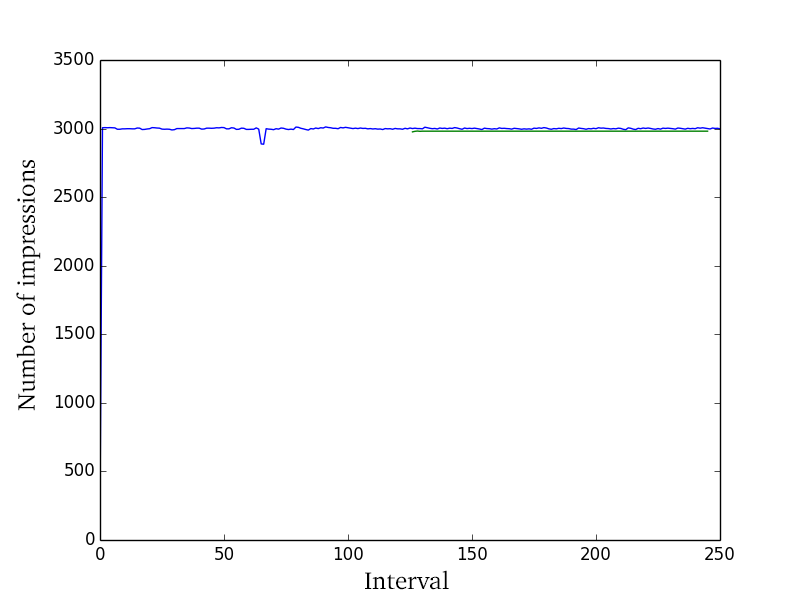
\includegraphics[width=0.96\textwidth]{forecast_12_wo_clustering} \caption[Volume
impression forecast, safari]{Volume impression
forecast, using 12h period without clustering (blue: real; green: forecast)}
\label{fig:vol_safari_12h_wo_clustering}
\end{minipage}
\quad
\begin{minipage}[t]{0.45\linewidth}
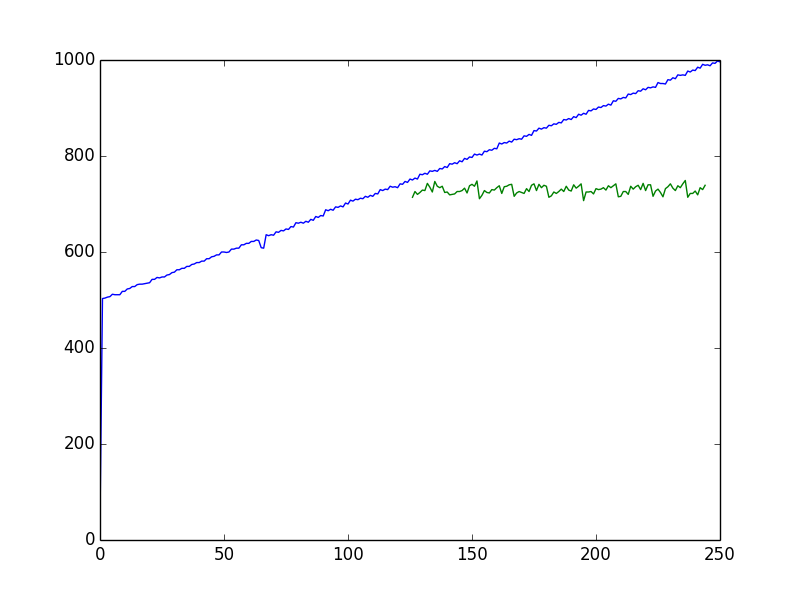
\includegraphics[width=0.96\textwidth]{safari4_wo_clustering_12} \caption[Volume
impression forecast, safari 4, without segmentation]{Volume impression
forecast, using 12h period without clustering, filtered by "Safari 4.0" (blue: real; green: forecast)}
\label{fig:vol_safari_12h_wo_clustering_safari_4} 
\end{minipage}
\end{figure}



\begin{table}[!ht]
\centering
\footnotesize
\begin{minipage}[t]{0.45\linewidth}
\centering
\begin{tabular}{ccc}
 $\sigma$ (Real Data) & RMSE & MASE   \\ \hline
 3.33      & 19.61        & 0.6760   \\
\end{tabular}

\vspace{0.5cm}

\caption[Volume
impression forecast error, safari]{Error for impression volume
forecast, using a 12h period without clustering}
\label{tab:err_forecast_12_safari}
\end{minipage}
\quad
\begin{minipage}[t]{0.45\linewidth}
\centering
\begin{tabular}{ccc}
 $\sigma$ (Real Data) & RMSE & MASE   \\ \hline
72.28      &  155.42       & 19.5770   \\
\end{tabular}

\vspace{0.5cm}

\caption[Volume
impression forecast error, safari, without segmentation]{Error for impression volume
forecast, using a 12h period without clustering, query for ''Safari 4.0''}
\label{tab:err_forecast_12_safari_wo_clustering_safari_4}

\end{minipage}
\end{table}

As shown in the figure~\ref{fig:vol_safari_12h_wo_clustering} and in the
table~\ref{tab:err_forecast_12_safari}, (without the segmentation phase) the
proposed approach was able to forecast the total volume of impressions only with
a small error.

In order to be able to see the result of the approach for the behavior of the
''Safari 4.0'' users we need to generate a future dataset (last phase of the
approach). The result for the query for the ''Safari 4.0'' browser, over the
resultant dataset, can be seen
on figure~\ref{fig:vol_safari_12h_wo_clustering_safari_4}.

As shown on the figure~\ref{fig:vol_safari_12h_wo_clustering_safari_4}, the
dataset generation phased mimics the behavior of that particular characteristic
from the previous week into the future, which in this case is not a good result.

\subsection*{Clustering Baseline}

In order to better compare the results of the different segmentation approaches,
a baseline method was used\footnote{the original dataset was grouped in a
chronological order on 100 different groups.}.

\begin{figure}[!ht]
\centering
\begin{minipage}[t]{0.45\linewidth}
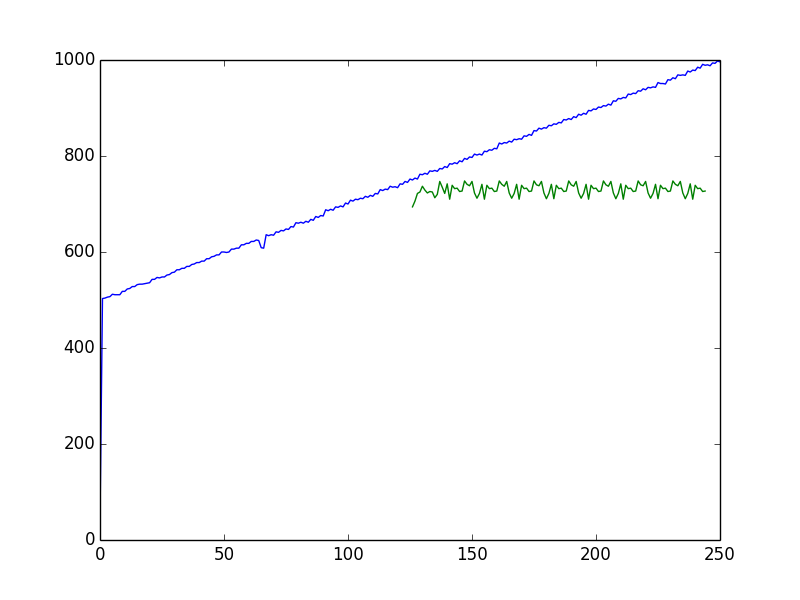
\includegraphics[width=0.96\textwidth]{forecast_12_w_clustering_baseline} \caption[Volume
impression forecast, safari 4, baseline clustering]{Volume impression
forecast, using 12h period with baseline clustering  (blue: real; green: forecast)}
\label{fig:vol_safari_12h_w_clustering_baseline}
\end{minipage}
\quad
\begin{minipage}[t]{0.45\linewidth}
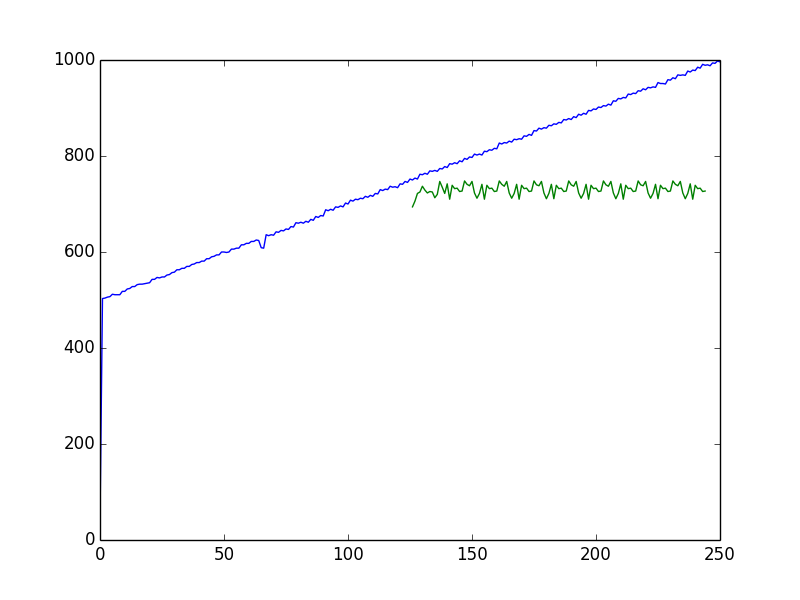
\includegraphics[width=0.96\textwidth]{forecast_12_w_clustering_baseline_safari4} \caption[Volume
impression forecast, safari 4, baseline clustering, filtered]{Volume impression
forecast, using 12h period with baseline clustering, filtered by "Safari 4.0" (blue: real; green: forecast)}
\label{fig:vol_safari_12h_w_clustering_baseline_safari_4}
\end{minipage}

\end{figure}

\begin{table}[!ht]
\centering
\footnotesize
\begin{minipage}[t]{0.45\linewidth}
\centering
\footnotesize
\begin{tabular}{ccc}
 $\sigma$ (Real Data) & RMSE & MASE   \\ \hline
3.33 & 3.38 & 0.0931 \\
\end{tabular}

\vspace{0.5cm}

\caption[Volume
impression forecast error, safari, baseline clustering]{Error for impression volume
forecast, using 12h period with baseline clustering}
\label{tab:err_forecast_12_safari_w_clustering_datastream_14}
\end{minipage}
\quad
\begin{minipage}[t]{0.45\linewidth}
\centering
\footnotesize
\begin{tabular}{ccc}
 $\sigma$ (Real Data) & RMSE & MASE   \\ \hline
72.28 & 154.99 & 19.5144 \\
\end{tabular}

\vspace{0.5cm}

\caption[Volume
impression forecast error, safari, baseline clustering, filtered]{Error for impression volume
forecast, using 12h period with baseline clustering, filtered by "Safari 4.0"}
\label{tab:err_forecast_12_safari_w_clustering_baseline_safari}
\end{minipage}

\end{table}

On figure~\ref{fig:vol_safari_12h_w_clustering_baseline} and table~\ref{tab:err_forecast_12_safari_w_clustering_baseline_safari}
we can assess that this approach gets a slight improvement over the
non-segmented approach. If we look at the filtered data
(Figure~\ref{fig:vol_safari_12h_w_clustering_baseline_safari_4}) the improvement
is not that noticeable.


\subsection*{Segmentation by Parameter}

\subsubsection*{Segmentation by browser}

Since we know that this particular dataset has a peculiarity, as previously seen
on filtered results (for example Figure~\ref{fig:vol_safari_12h_w_clustering_safari_4}), in the browser
parameter impression volume. To verify how the prediction would react to the clustering by
parameter(specifically by the browser attribute) this will forecast the volumes
values for each browser present on the dataset. This allow us to get better results in
predicting the traffic volumes for each browser.

As we can see on Figure~\ref{fig:vol_safari_12h_w_clustering}, the overall error
(Table~\ref{tab:err_forecast_12_safari_w_clustering}) for impression volume
forecasting is worse than without the clustering phase. This is due to the fact that the prediction error
associated with each cluster is amplified when the volume data is joined
back together.

\begin{figure}[!ht]
\centering
\begin{minipage}[b]{0.45\linewidth}
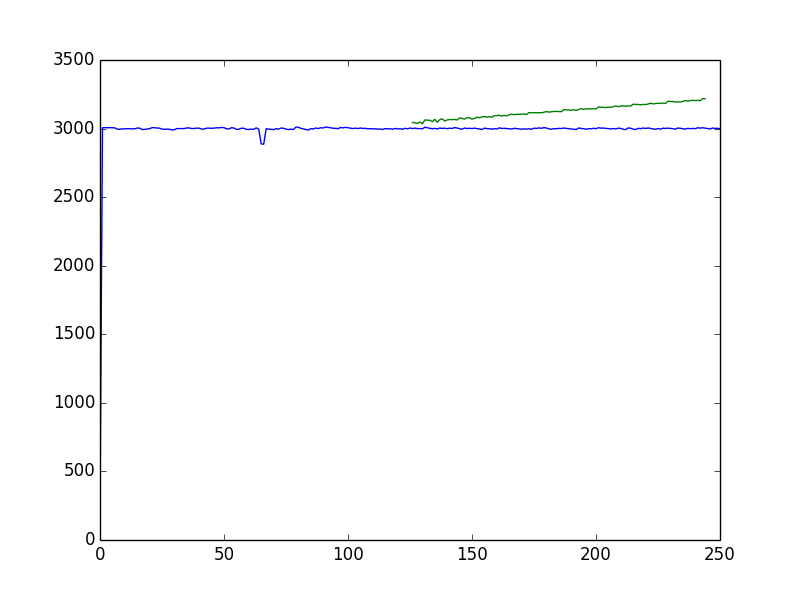
\includegraphics[width=0.96\textwidth]{forecast_12_w_clustering_per_browser} \caption[Volume
impression forecast, safari 4, clustering by browser]{Volume impression
forecast, using 12h period with clustering by the browser attribute (blue: real; green: forecast)}
\label{fig:vol_safari_12h_w_clustering}
\end{minipage}
\quad
\begin{minipage}[b]{0.45\linewidth}
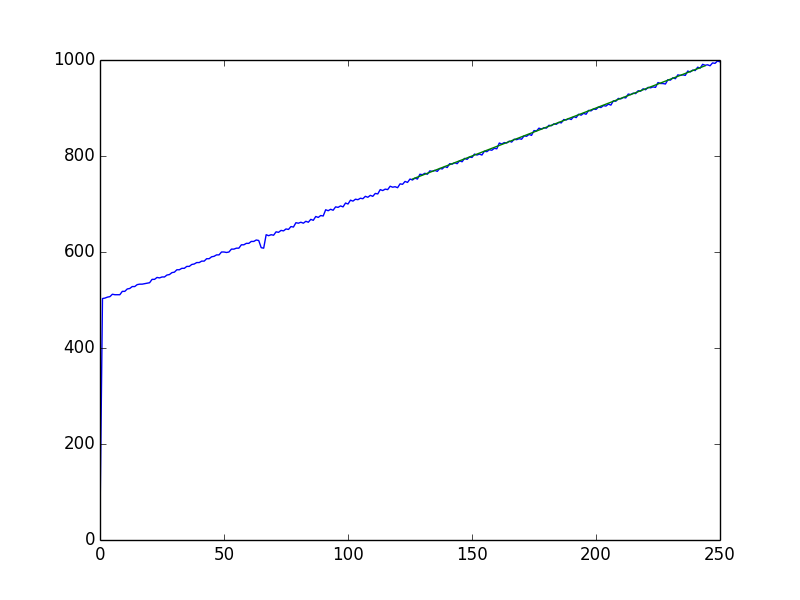
\includegraphics[width=0.96\textwidth]{safari4_w_clustering_12} \caption[Volume
impression forecast, safari 4, clustering by browser, filtered]{Volume impression
forecast, using 12h period with clustering by the browser parameter, filtered by "Safari 4.0" (blue: real; green: forecast)}
\label{fig:vol_safari_12h_w_clustering_safari_4}
\end{minipage}

\end{figure}

\begin{table}[!ht]
\centering
\footnotesize
\begin{minipage}[t]{0.45\linewidth}
\centering

\footnotesize
\begin{tabular}{ccc}
 $\sigma$ (Real Data) & RMSE & MASE   \\ \hline
3.33 & 136.78 & 4.4253 \\
\end{tabular}

\vspace{0.5cm}

\caption[Volume
impression forecast error, safari, clustering by browser]{Error for impression volume
forecast, using a 12h period with clustering by browser attribute}
\label{tab:err_forecast_12_safari_w_clustering}
\end{minipage}
\quad
\begin{minipage}[t]{0.45\linewidth}
\centering
\footnotesize
\begin{tabular}{ccc}
 $\sigma$ (Real Data) & RMSE & MASE   \\ \hline
72.28 & 2.58 & 0.2892 \\
\end{tabular}

\vspace{0.5cm}

\caption[Volume
impression forecast error, safari, clustering by browser, filtered]{Error for impression volume
forecast, using a 12h period with clustering by browser attribute, query for ''Safari 4.0''}
\label{tab:err_forecast_12_safari_w_clustering_safari_4}

\end{minipage}

\end{table}

In the other hand, in the
Figure~\ref{fig:vol_safari_12h_w_clustering_safari_4}(which show the results
filtered by ''Safari 4.0'' browser) we get a better result prediction for this
characteristic, as shown by the error values on
Table~\ref{tab:err_forecast_12_safari_w_clustering_safari_4}.
This tells us that \emph{clustering by parameter} gives better predictions for certain
characteristics, by capturing the volume for each one in the past and
propagating it into the future.

\subsection*{Using datastream-based clustering}

\begin{figure}[!ht]
\centering
\begin{minipage}[t]{0.45\linewidth}
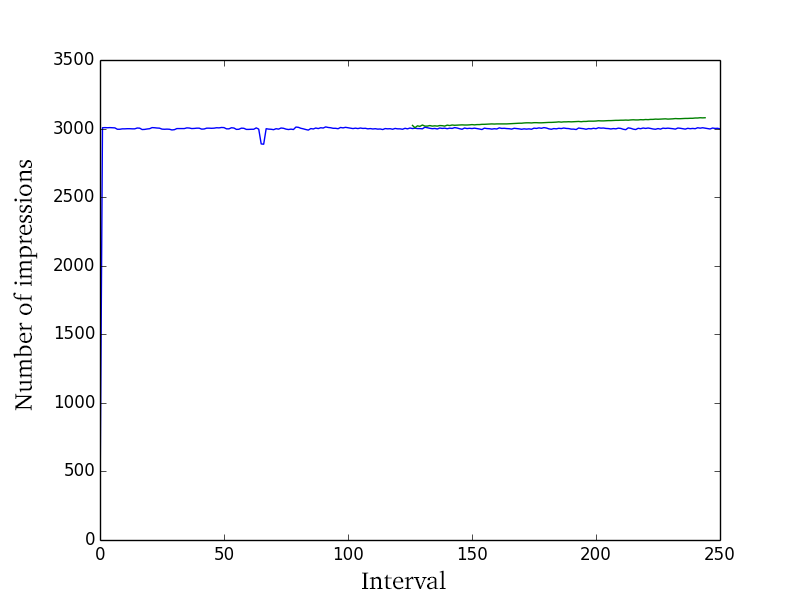
\includegraphics[width=0.96\textwidth]{forecast_12_w_clustering_datastream_14} \caption[Volume
impression forecast, safari 4, datastream]{Volume impression
forecast, using 12h period with clustering based datastream-based clustering,
with a \emph{threshold} of 14 maximum distance  (blue: real; green: forecast)}
\label{fig:vol_safari_12h_w_clustering_datastream_14}
\end{minipage}
\quad
\begin{minipage}[t]{0.45\linewidth}
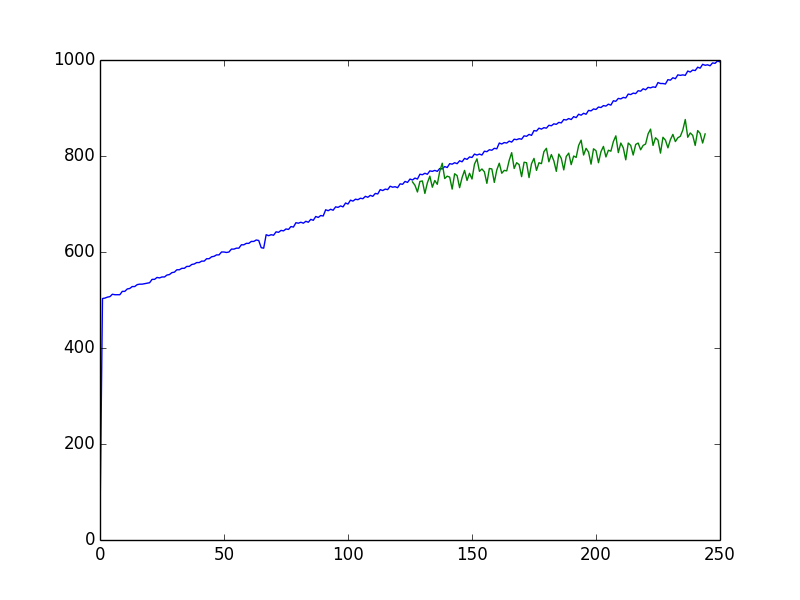
\includegraphics[width=0.96\textwidth]{safari4_w_clustering_12_datastream14} \caption[Volume
impression forecast, safari 4, datastream, filtered]{Volume impression
forecast, using 12h period with clustering based datastream-based clustering,
with a \emph{threshold} of 14 maximum distance, filtered by "Safari 4.0" (blue: real; green: forecast)}
\label{fig:vol_safari_12h_w_clustering_datastream_14_safari_4}
\end{minipage}

\end{figure}

\begin{table}[!ht]
\centering
\footnotesize
\begin{minipage}[t]{0.45\linewidth}
\centering
\footnotesize
\begin{tabular}{ccc}
 $\sigma$ (Real Data) & RMSE & MASE   \\ \hline
3.33 & 50.41 & 1.6226 \\
\end{tabular}

\vspace{0.5cm}

\caption[Volume
impression forecast error, safari, datastream]{Error for impression volume
forecast, using 12h period with clustering based datastream-based clustering,
with a \emph{threshold} of 14 maximum distance }
\label{tab:err_forecast_12_safari_w_clustering_datastream_14}
\end{minipage}
\quad
\begin{minipage}[t]{0.45\linewidth}
\centering
\footnotesize
\begin{tabular}{ccc}
 $\sigma$ (Real Data) & RMSE & MASE   \\ \hline
72.28 & 84.78 & 10.5275 \\
\end{tabular}

\vspace{0.5cm}

\caption[Volume
impression forecast error, safari, datastream, filtered]{Error for impression volume
forecast, using 12h period with clustering based datastream-based clustering,
with a \emph{threshold} of 14 maximum distance, filtered by "Safari 4.0"}
\label{tab:err_forecast_12_safari_w_clustering_datastream_14}
\end{minipage}

\end{table}

Using the datastream-based clustering method, with a \emph{threshold} of 14
(which means that each group member of each groups will only have a maximum of 14
parameters different than the centroid of the group) the result for the overall
impressions volume was worse than methods without clustering and the baseline clustering
method, but better than the clustering by browser. If we analyse the
figure~\ref{fig:vol_safari_12h_w_clustering_datastream_14_safari_4}, we can
assess than the result is only beat by the clustering for that specific
parameter, which ultimately is a good result.

\subsection{Specific Domain decreasing linearly}

For this set of tests another artificially generated dataset was used, in this
particular case one of the domains represented on the dataset, with a steady linear decrease following a linear function.

\subsection*{Without Segmentation}

\begin{figure}[!ht]
\centering
\begin{minipage}[t]{0.45\linewidth}
\includegraphics[width=0.96\textwidth]{results_3/wo_clustering} \caption[Volume
impression forecast, without segmentation]{Impression volume
forecast, using 12h period without segmentation (blue: real; green: forecast)}
\label{fig:vol_domain_wo_segmentation}
\end{minipage}
\quad
\begin{minipage}[t]{0.45\linewidth}
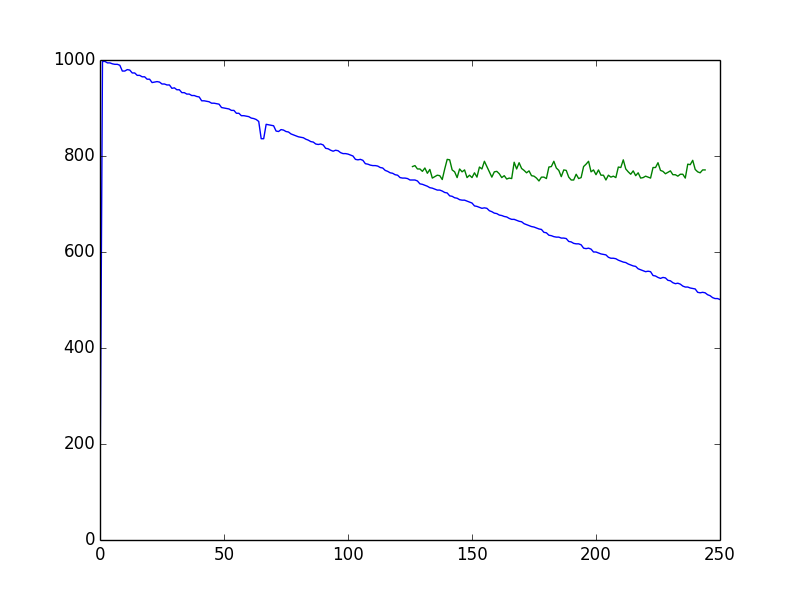
\includegraphics[width=0.96\textwidth]{results_3/host_wo_clustering} \caption[Volume
impression forecast, without segmentation]{Impression volume
forecast, using 12h period without segmentation, filtered by the domain ''ef4e08fb71d96d19406663f8bb7ce6c0'' (blue: real; green: forecast)}
\label{fig:vol_domain_wo_segmentation_filtered}
\end{minipage}

\end{figure}

\begin{table}[!ht]
\centering
\footnotesize
\begin{minipage}[t]{0.45\linewidth}
\centering
\footnotesize
\begin{tabular}{ccc}
 $\sigma$ (Real Data) & RMSE & MASE   \\ \hline
4.33 & 5.00 & 0.1392 \\
\end{tabular}

\vspace{0.5cm}

\caption[Volume
impression forecast, safari]{Error for impression volume
forecast, using 12h period without segmentation }
\label{tab:err_domain_wo_segmentation}
\end{minipage}
\quad
\begin{minipage}[t]{0.45\linewidth}
\centering
\footnotesize
\begin{tabular}{ccc}
 $\sigma$ (Real Data) & RMSE & MASE   \\ \hline
72.50 & 152.78 & 12.8542 \\
\end{tabular}

\vspace{0.5cm}

\caption[Volume
impression forecast, safari]{Error for impression volume
forecast, using 12h period without segmentation, filtered by the domain ''ef4e08fb71d96d19406663f8bb7ce6c0'' }
\label{tab:err_domain_wo_segmentation_filtered}
\end{minipage}

\end{table}

Without any segmentation phase we obtained a good result for the overall
impression volume prediction. If we filter the results for the particular
domain
that we know will be decreasing, the result mimics the behaviour of the previous
weeks since the information about that particular domain is limited.

\subsection*{Clustering Baseline}

\begin{figure}[!ht]
\centering
\begin{minipage}[t]{0.45\linewidth}
\includegraphics[width=0.96\textwidth]{results_3/baseline} \caption[Volume
impression forecast, domain, cluster by baseline]{Impression volume
forecast, using 12h period using baseline segmentation  (blue: real; green: forecast)}
\label{fig:domain_w_baseline}
\end{minipage}
\quad
\begin{minipage}[t]{0.45\linewidth}
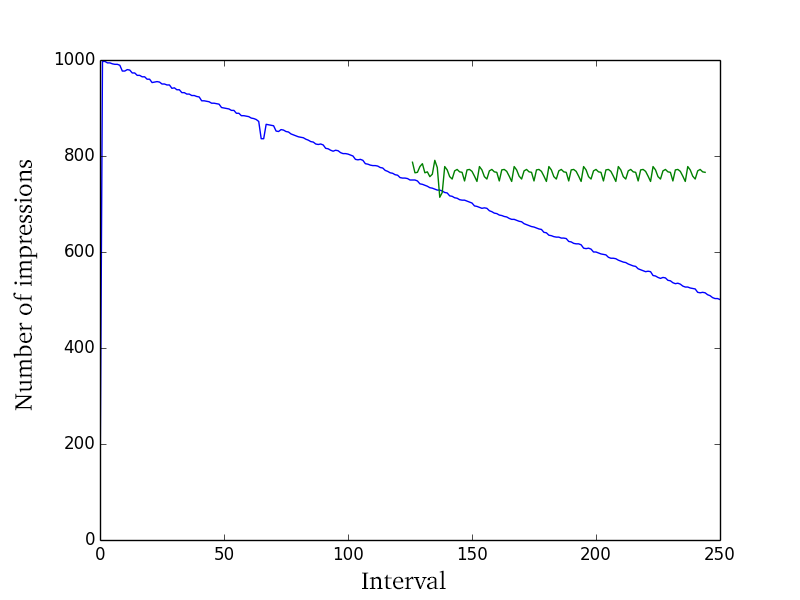
\includegraphics[width=0.96\textwidth]{results_3/host_baseline} \caption[Volume
impression forecast, domain, cluster by baseline, filtered]{Impression volume
forecast, using 12h period using baseline segmentation, filtered by the domain ''ef4e08fb71d96d19406663f8bb7ce6c0'' (blue: real; green: forecast)}
\label{fig:domain_w_baseline_filtered}
\end{minipage}

\end{figure}

\begin{table}[!ht]
\centering
\footnotesize
\begin{minipage}[t]{0.45\linewidth}
\centering
\footnotesize
\begin{tabular}{ccc}
 $\sigma$ (Real Data) & RMSE & MASE   \\ \hline
4.33 & 4.30 & 0.1176 \\
\end{tabular}

\vspace{0.5cm}

\caption[Error Volume
impression forecast, domain, filtered]{Error for impression volume
forecast, using 12h period with baseline segmentation}
\label{tab:err_domain_w_segmentation_baseline}
\end{minipage}
\quad
\begin{minipage}[t]{0.45\linewidth}
\centering
\footnotesize
\begin{tabular}{ccc}
 $\sigma$ (Real Data) & RMSE & MASE   \\ \hline
72.50 & 150.7442 & 12.6627 \\
\end{tabular}

\vspace{0.5cm}

\caption[Error Volume
impression forecast, domain, filtered]{Error for impression volume
forecast, using 12h period with baseline segmentation, filtered by the domain ''ef4e08fb71d96d19406663f8bb7ce6c0'' }
\label{tab:err_domain_w_segmentation_baseline_filtered}
\end{minipage}

\end{table}


In the figure~\ref{fig:domain_w_baseline} and
table~\ref{tab:err_domain_w_segmentation_baseline} we can take a look at the
results given by the segmentation baseline method for the total volume of
impressions forecast for this dataset. The figures show the results are better
than without segmentation, and when we filter the data for the domain that is
decreasing in volume of impressions (figure~\ref{fig:domain_w_baseline_filtered}
and table~\ref{tab:err_domain_w_segmentation_baseline_filtered}) we also obtain
a slightly better result.

\subsection*{Segmentation by Parameter}

\subsubsection*{Segmentation by Domain}

\begin{figure}[!ht]
\centering
\begin{minipage}[t]{0.45\linewidth}
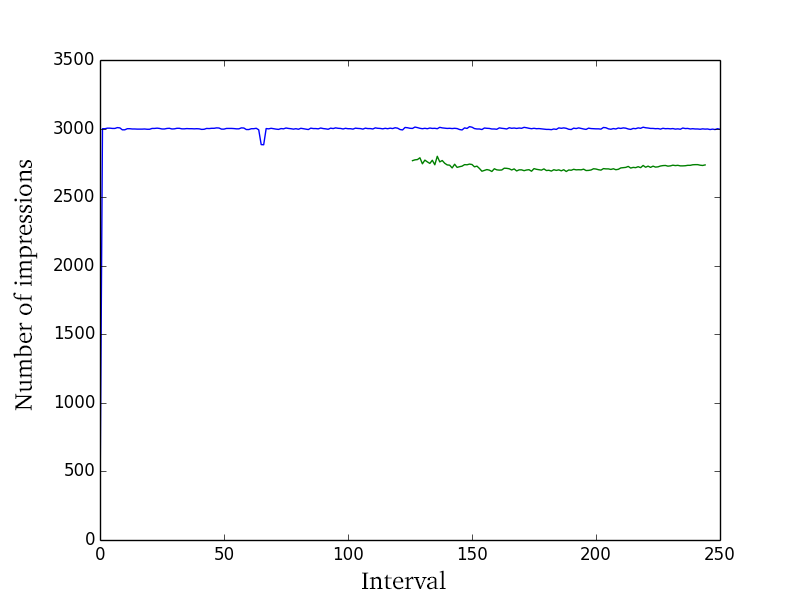
\includegraphics[width=0.96\textwidth]{results_3/per_host}

\caption[Volume
impression forecast, domain, cluster by domain]{Impression volume
forecast, using 12h period using segmentation by domain (blue: real; green: forecast)}
\label{fig:domain_w_domain}


\end{minipage}
\quad
\begin{minipage}[t]{0.45\linewidth}
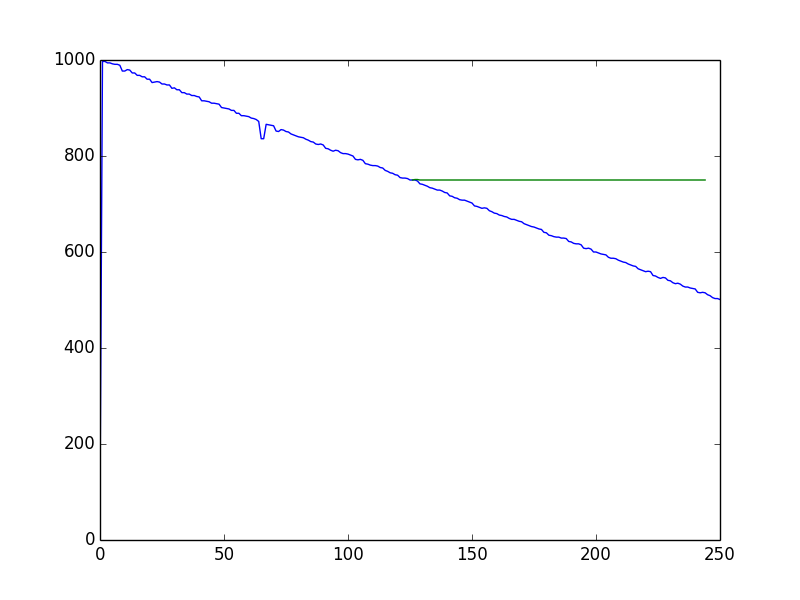
\includegraphics[width=0.96\textwidth]{results_3/host_per_host} 
\caption[Volume
impression forecast, domain, cluster by domain, filtered]{Impression volume
forecast, using 12h period using segmentation by domain, filtered by the domain ''ef4e08fb71d96d19406663f8bb7ce6c0'' (blue: real; green: forecast)}
\label{fig:domain_w_domain_filtered}

\end{minipage}

\end{figure}

\begin{table}[!ht]
\centering
\footnotesize
\begin{minipage}[t]{0.45\linewidth}
\centering
\footnotesize
\begin{tabular}{ccc}
 $\sigma$ (Real Data) & RMSE & MASE   \\ \hline
4.33 & 283.20 & 9.9304 \\
\end{tabular}

\vspace{0.5cm}

\caption[Error Volume
impression forecast, domain]{Error for impression volume
forecast, using 12h period with segmentation by domain}
\label{tab:err_domain_w_segmentation_domain}


\end{minipage}
\quad
\begin{minipage}[t]{0.45\linewidth}
\centering
\footnotesize
\begin{tabular}{ccc}
 $\sigma$ (Real Data) & RMSE & MASE   \\ \hline
72.50 & 137.93 & 11.2913 \\
\end{tabular}

\vspace{0.5cm}

\caption[Error Volume
impression forecast, domain, filtered]{Error for impression volume
forecast, using 12h period with segmentation by domain, filtered by the domain ''ef4e08fb71d96d19406663f8bb7ce6c0'' }
\label{tab:err_domain_w_segmentation_domain_filtered}


\end{minipage}

\end{table}

Like we did for the previous test group (where we knew that a particular browser
was increasing its value in volume impressions and so we segmented the data by
browser),
in this case we know that a domain is decreasing, so we tested segment the data
by domain. In the figure~\ref{fig:domain_w_domain_filtered} the results were
not as expected. Even though we got a better result in the filtered data, when
compared to the previous methods, the result for the total volume is
much worse. This is probably due to the small volumes in each domain, since in this
dataset there was about 4300 domains in around 3000 impressions for each 12h
period,
which can result in a very difficult to predict time series.


\subsection*{Using datastream-based clustering}

\begin{figure}[!ht]
\centering
\begin{minipage}[t]{0.45\linewidth}
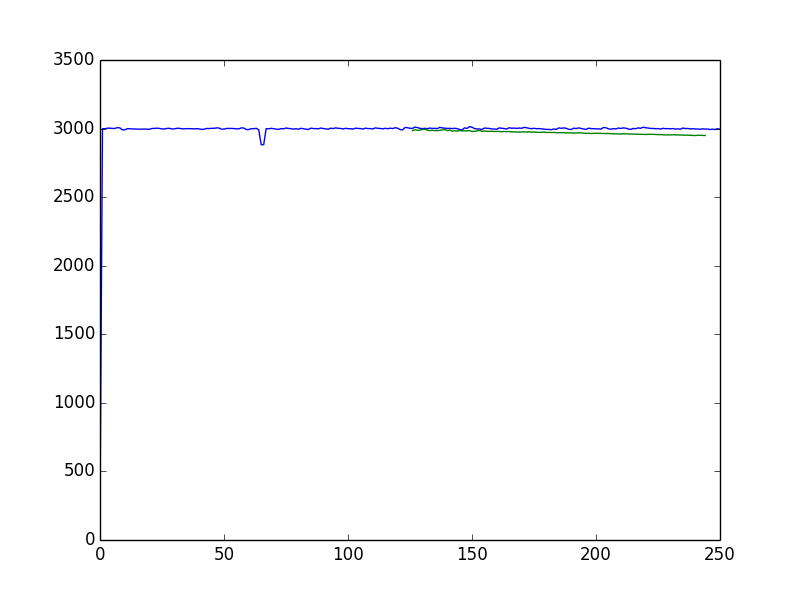
\includegraphics[width=0.96\textwidth]{results_3/datastream_14} 
\caption[Volume
impression forecast, domain, cluster by datastream]{Impression volume
forecast, using 12h period using datastream-based clustering with a
\emph{threshold} of 14 (blue: real; green: forecast)}
\label{fig:domain_w_datastream}

\end{minipage}
\quad
\begin{minipage}[t]{0.45\linewidth}
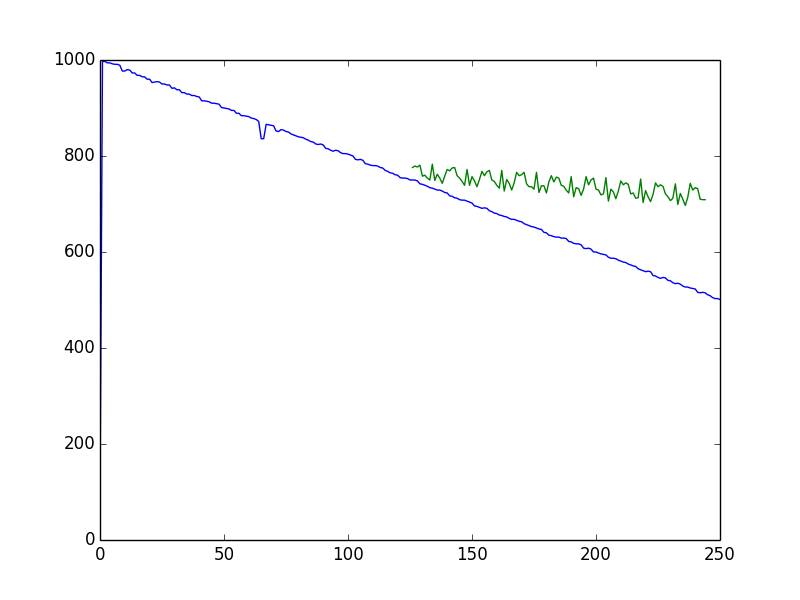
\includegraphics[width=0.96\textwidth]{results_3/host_datastream_14.png} 
\caption[Volume
impression forecast, domain, cluster by datastream, filtered]{Impression volume
forecast, using 12h period using datastream-based clustering with a
\emph{threshold} of 14, filtered by the domain ''ef4e08fb71d96d19406663f8bb7ce6c0'' (blue: real; green: forecast)}
\label{fig:domain_w_datastream_filtered}

\end{minipage}

\end{figure}

\begin{table}[!ht]
\centering
\footnotesize
\begin{minipage}[t]{0.45\linewidth}
\centering
\footnotesize
\begin{tabular}{ccc}
 $\sigma$ (Real Data) & RMSE & MASE   \\ \hline
4.33 & 32.48 & 1.0613 \\
\end{tabular}

\vspace{0.5cm}

\caption[Error Volume
impression forecast, datastream, filtered]{Error for impression volume
forecast, using 12h period using datastream-based clustering with a
\emph{threshold} of 14}
\label{tab:err_domain_w_datastream}


\end{minipage}
\quad
\begin{minipage}[t]{0.45\linewidth}
\centering
\footnotesize
\begin{tabular}{ccc}
 $\sigma$ (Real Data) & RMSE & MASE   \\ \hline
72.50 & 123.27 & 10.3919 \\
\end{tabular}

\vspace{0.5cm}

\caption[Error Volume
impression forecast, domain, filtered]{Error for impression volume
forecast, using 12h period using datastream-based clustering with a
\emph{threshold} of 14, filtered by the domain ''ef4e08fb71d96d19406663f8bb7ce6c0'' }
\label{tab:err_domain_w_segmentation_datastream_filtered}


\end{minipage}

\end{table}

The datastream-based segmentation approach using a \emph{threshold} equal to 14 of
maximum distance, we get a slightly worse result than the method without segmentation and
the baseline segmentation approach, as shown by
Figure~\ref{fig:domain_w_datastream} and
Table~\ref{tab:err_domain_w_datastream}. This is the method responsible for the best results on this series,
in terms of capturing the peculiarity of this
dataset, as shown by figure~\ref{fig:domain_w_datastream_filtered} and
table~\ref{tab:err_domain_w_segmentation_datastream_filtered}.

\subsection{Real Data}

For this last series of tests we used a dataset containing real data. Since we
don't know any particular characteristic to search for, we will compare the
results for the query for ''Portugal'' as country of origin for each impression.

\subsection*{Without Segmentation}

\begin{figure}[!ht]
\centering
\begin{minipage}[t]{0.45\linewidth}
\includegraphics[width=0.96\textwidth]{results_real/wo_clustering}
\caption[Volume
impression forecast, real data]{Impression volume
forecast, using 12h period without clustering (blue: real; green: forecast)}
\label{fig:vol_real_data_wo_clustering}
\end{minipage}
\quad
\begin{minipage}[t]{0.45\linewidth}
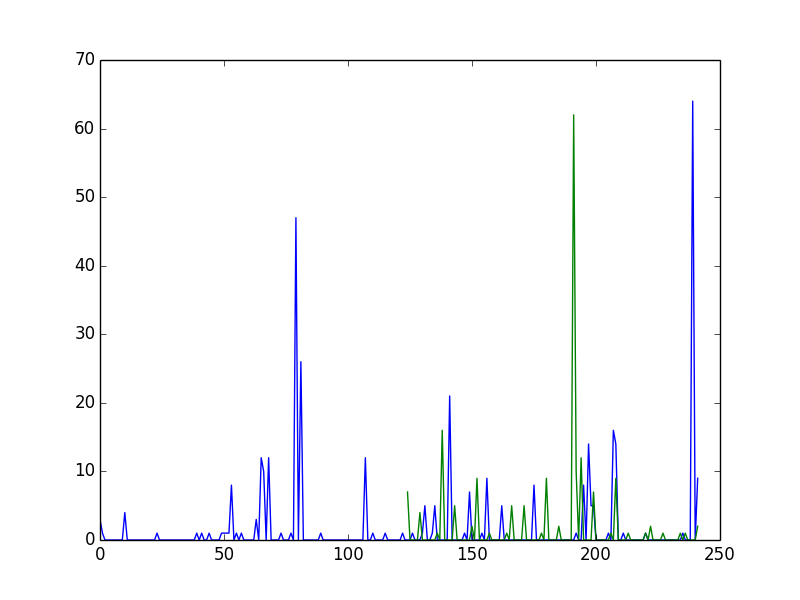
\includegraphics[width=0.96\textwidth]{results_real/wo_clustering_portugal} \caption[Volume
impression forecast, real data, Portugal]{Impression volume
forecast, using 12h period without clustering, filtered by country = Portugal (blue: real; green: forecast)}
\label{fig:vol_real_data_wo_clustering_filtered}
\end{minipage}

\end{figure}

\begin{table}[!ht]
\centering
\footnotesize
\begin{minipage}[t]{0.45\linewidth}
\centering
\footnotesize
\begin{tabular}{ccc}
 $\sigma$ (Real Data) & RMSE & MASE   \\ \hline
2224.74 & 1237.99 & 0.1958 \\
\end{tabular}

\vspace{0.5cm}

\caption[Volume
impression forecast, real data, without clustering]{Error for impression volume
forecast, using 12h period without clustering}
\label{tab:err_real_data_wo_clustering}
\end{minipage}
\quad
\begin{minipage}[t]{0.45\linewidth}
\centering
\footnotesize
\begin{tabular}{ccc}
 $\sigma$ (Real Data) & RMSE & MASE   \\ \hline
6.70 & 9.24 & 1.2511 \\
\end{tabular}

\vspace{0.5cm}

\caption[Volume
impression forecast, safari]{Error for impression volume
forecast, using 12h period without clustering, filtered by country = Portugal}
\label{tab:err_real_data_wo_clustering_filtered}
\end{minipage}

\end{table}

Like in the other datasets we start by testing the result without any
segmentation. In overall volume of impressions we get a good result
(figure~\ref{fig:vol_real_data_wo_clustering} and
table~\ref{tab:err_real_data_wo_clustering}), and when over the result a query
for origin country ''Portugal'' is done, the result mimics the past
characteristics and the result on this case is not bad.


\subsection*{Clustering Baseline}

\begin{figure}[!ht]
\centering
\begin{minipage}[t]{0.45\linewidth}
\includegraphics[width=0.96\textwidth]{results_real/baseline} \caption[Volume
impression forecast, real data, clustering baseline]{Impression Volume 
forecast, using 12h period with baseline segmentation (blue: real; green: forecast)}
\label{fig:vol_real_data_baseline}
\end{minipage}
\quad
\begin{minipage}[t]{0.45\linewidth}
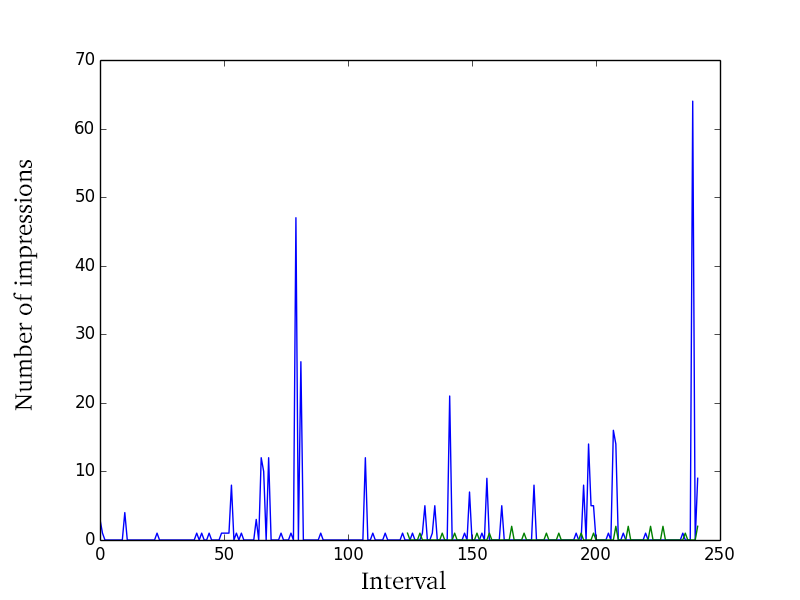
\includegraphics[width=0.96\textwidth]{results_real/baseline_portugal} \caption[Volume
impression forecast, real data, clustering baselinei, filtered]{Impression Volume 
forecast, using 12h period with baseline segmentation, filtered by country =
Portugal (blue: real; green: forecast)}
\label{fig:vol_real_data_baseline_filtered}
\end{minipage}

\end{figure}

\begin{table}[!ht]
\centering
\footnotesize
\begin{minipage}[t]{0.45\linewidth}
\centering
\footnotesize
\begin{tabular}{ccc}
 $\sigma$ (Real Data) & RMSE & MASE   \\ \hline
2224.74 & 1352.42 & 0.2174 \\
\end{tabular}

\vspace{0.5cm}

\caption[Volume
impression forecast, baseline]{Error for volume impression forecast, using 12h
period with baseline clustering}
\label{tab:err_forecast_12_real_data_baseline}
\end{minipage}
\quad
\begin{minipage}[t]{0.45\linewidth}
\centering
\footnotesize
\begin{tabular}{ccc}
 $\sigma$ (Real Data) & RMSE & MASE   \\ \hline
6.70 & 6.88 & 0.7896 \\
\end{tabular}

\vspace{0.5cm}

\caption[Volume
impression forecast, safari]{Error for impression volume
forecast, using 12h period with baseline clustering, filtered by country =
Portugal}
\label{tab:err_forecast_12_real_data_baseline_filtered}
\end{minipage}

\end{table}

In this case the baseline segmentation gets a worse result than the
non-segmented approach in terms of total volume, but a better approximation
in terms of the results for the query ''Portugal''. This is probably due to additional
granularity gained by the data division.


\subsection*{Segmentation by Parameter}

\subsubsection*{Segmentation by browser}

\begin{figure}[!ht]
\centering
\begin{minipage}[t]{0.45\linewidth}
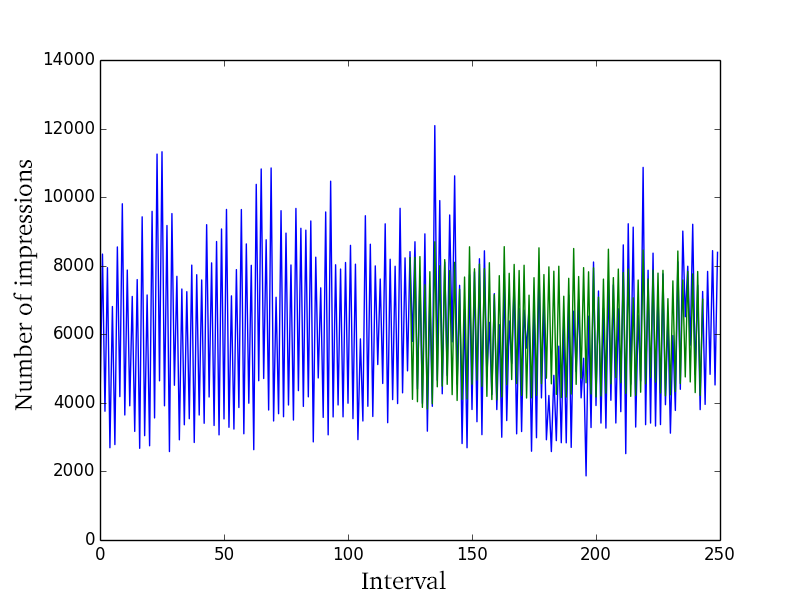
\includegraphics[width=0.96\textwidth]{results_real/perbrowser} \caption[Volume
impression forecast, real data, clustering by browser]{Impression Volume 
forecast, using 12h period with segmentation by browser(blue: real; green: forecast)}
\label{fig:vol_real_data_browser}
\end{minipage}
\quad
\begin{minipage}[t]{0.45\linewidth}
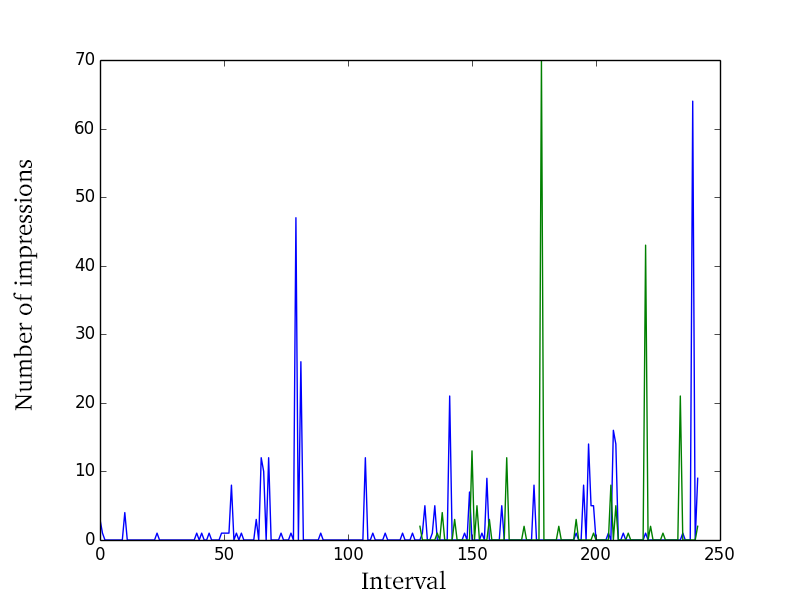
\includegraphics[width=0.96\textwidth]{results_real/perbrowser_portugal}\caption[Volume
impression forecast, real data, clustering by browser, filtered]{Impression Volume 
forecast, using 12h period with segmentation by browser, filtered by country =
Portugal (blue: real; green: forecast)}
\label{fig:vol_real_data_browser_filtered}
\end{minipage}

\end{figure}

\begin{table}[!ht]
\centering
\footnotesize
\begin{minipage}[t]{0.45\linewidth}
\centering
\footnotesize
\begin{tabular}{ccc}
 $\sigma$ (Real Data) & RMSE & MASE   \\ \hline
2224.74 & 1226.60 & 0.1884 \\
\end{tabular}

\vspace{0.5cm}

\caption[Volume
impression forecast, real data, browser]{Error for impression volume
forecast, using 12h period with segmentation by browser}
\label{tab:err_forecast_12_real_data_browser}
\end{minipage}
\quad
\begin{minipage}[t]{0.45\linewidth}
\centering
\footnotesize
\begin{tabular}{ccc}
 $\sigma$ (Real Data) & RMSE & MASE   \\ \hline
6.70 & 10.75 & 1.3883 \\
\end{tabular}

\vspace{0.5cm}

\caption[Volume
impression forecast, real data, browser, filtered]{Error for impression volume
forecast, using 12h period with segmentation by browser, filtered by country =
Portugal}
\label{tab:err_forecast_12_real_data_browser_filtered}
\end{minipage}

\end{table}

Since in the case of this dataset we do not know for which particular parameter
we might want to segment by, the browser parameter was randomly selected as the
segmentation parameter. For the overall volume result this was the best result
over the other approaches over this particular dataset. In terms of the query
for ''Portugal'' the result was slightly worse than the previous approaches.

\subsection*{Using datastream-based clustering}

\begin{figure}[!ht]
\centering
\begin{minipage}[t]{0.45\linewidth}
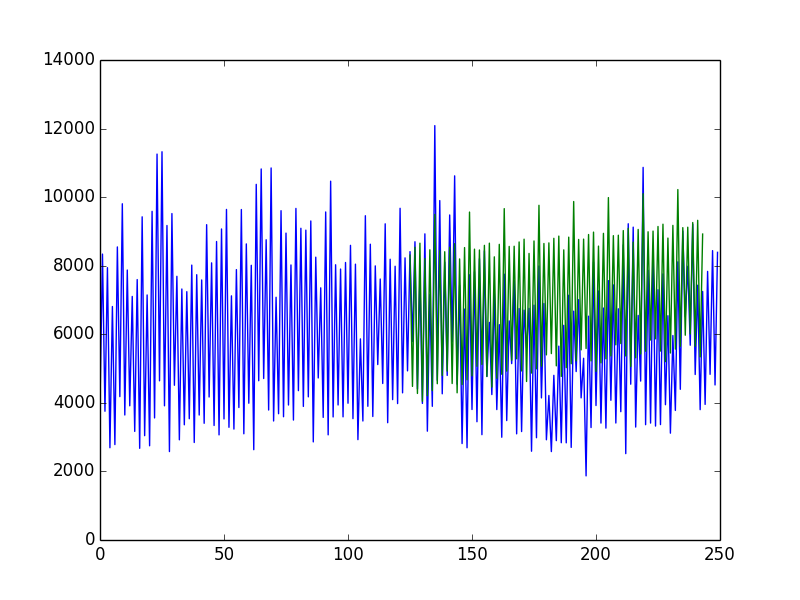
\includegraphics[width=0.96\textwidth]{results_real/datastream_20} \caption[Volume
impression forecast, real data, clustering datastream]{Impression Volume 
forecast, using 12h period with datastream-based segmentation using
\emph{threshold} of 20 (blue: real; green: forecast)}
\label{fig:vol_real_data_datastream}
\end{minipage}
\quad
\begin{minipage}[t]{0.45\linewidth}
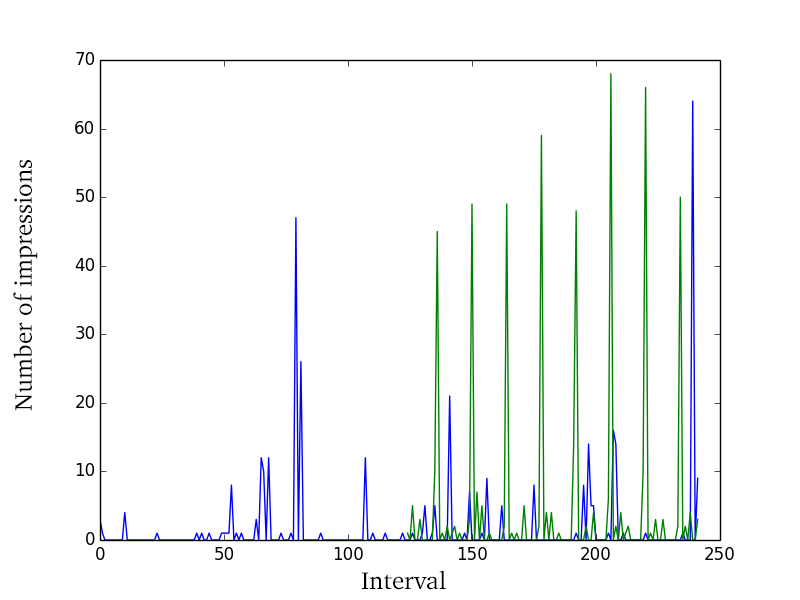
\includegraphics[width=0.96\textwidth]{results_real/datastream_20_portugal} \caption[Volume
impression forecast, real data, clustering datastream, filtered]{Volume impression
forecast, using 12h period with datastream-based segmentation using
\emph{threshold} of 20, filtered by country = Portugal  (blue: real; green: forecast)}
\label{fig:vol_real_data_datastream_filtered}
\end{minipage}

\end{figure}

\begin{table}[!ht]
\centering
\footnotesize
\begin{minipage}[t]{0.45\linewidth}
\centering
\footnotesize
\begin{tabular}{ccc}
 $\sigma$ (Real Data) & RMSE & MASE   \\ \hline
2224.74 & 1786.43 & 0.2927 \\
\end{tabular}

\vspace{0.5cm}

\caption[Volume
impression forecast, real data, datastream]{Error for impression volume
forecast, using 12h period with datastream-based segmentation using
\emph{threshold} of 20}
\label{tab:err_forecast_12_real_datastream_filtered}
\end{minipage}
\quad
\begin{minipage}[t]{0.45\linewidth}
\centering
\footnotesize
\begin{tabular}{ccc}
 $\sigma$ (Real Data) & RMSE & MASE   \\ \hline
6.70 & 15.93 & 2.5960 \\
\end{tabular}

\vspace{0.5cm}

\caption[Volume
impression forecast, real data, datastream, filtered]{Error for impression volume
forecast, using 12h period with datastream-based segmentation using
\emph{threshold} of 20, filtered by country = Portugal}
\label{tab:err_forecast_12_real_datastream_filtered}
\end{minipage}

\end{table}

For this dataset the \emph{threshold} for the distance needed to be increased to
20 (out of 28) because with a smaller \emph{threshold} we would get too many
groups, and some of them with data in the future were not represented on the training
dataset.

In overall analysis this was the worst result for this dataset for impression
volume forecast and for the queried data. This bad result is due to the fact that the results did not have
any particular characteristic in terms of
volume trend that made sense together, but were group because they had similar
parameters.

\section{Conclusion}

In about every test case, the results that used the segmentation phase got better
results.

These results were only compared to a small number of queries, so the results can
be completely different when used in its goal environment, the
online advertising campaigns impact on that particular network.

In order to be able to assess this impact a simulator should have been used to
test the results of this approach at its fully capability. But due to time
constraints this was not possible.
